\chapter{Common Lifetime Patterns}

It would be great if programmers could be in charge only of hooking together and
populating their data structures, leaving the \jre responsible for the details
of object allocation and reclamation. The Java runtime does indeed help manage some
aspects of these management tasks, but leaves a good deal of work in your hands.
In Java, you needn't explicitly free objects, and in that way a managed language
is a big step up from a language like C. However, the ultimate promise of
automatic memory management, that you can create objects without regard for messy
details of storage management, doesn't play out ideally in practice. Unless you
are careful, your program will suffer from bugs such as memory leaks, and suffer
from poor performance. Sometimes, your objects don't easily fit into the limits
of a single Java process, and you need to manage, explicitly, shuttling them in
and out of the Java heap.

When programming in Java it is important to plan out the lifetime of your
objects. \autoref{tab:five-lifetimes} summarizes five important cases of object
lifetime discussed in this chapter. Your application needs some objects to live
forever and it needs the rest to die a timely death. This often requires careful
design on your part, both to avoid bugs and so that your application performs
well in the case when not everything fits into the Java heap. These trickier
aspects of memory management, summarized in
\autoref{tab:tricky-memory-management}, are discussed in greater detail in later
chapters. Designing a lifetime management strategy usually requires that you take
the tools that Java provides, and combine them with other strategies implemented
on top of Java.

\begin{figure}
	\centering
	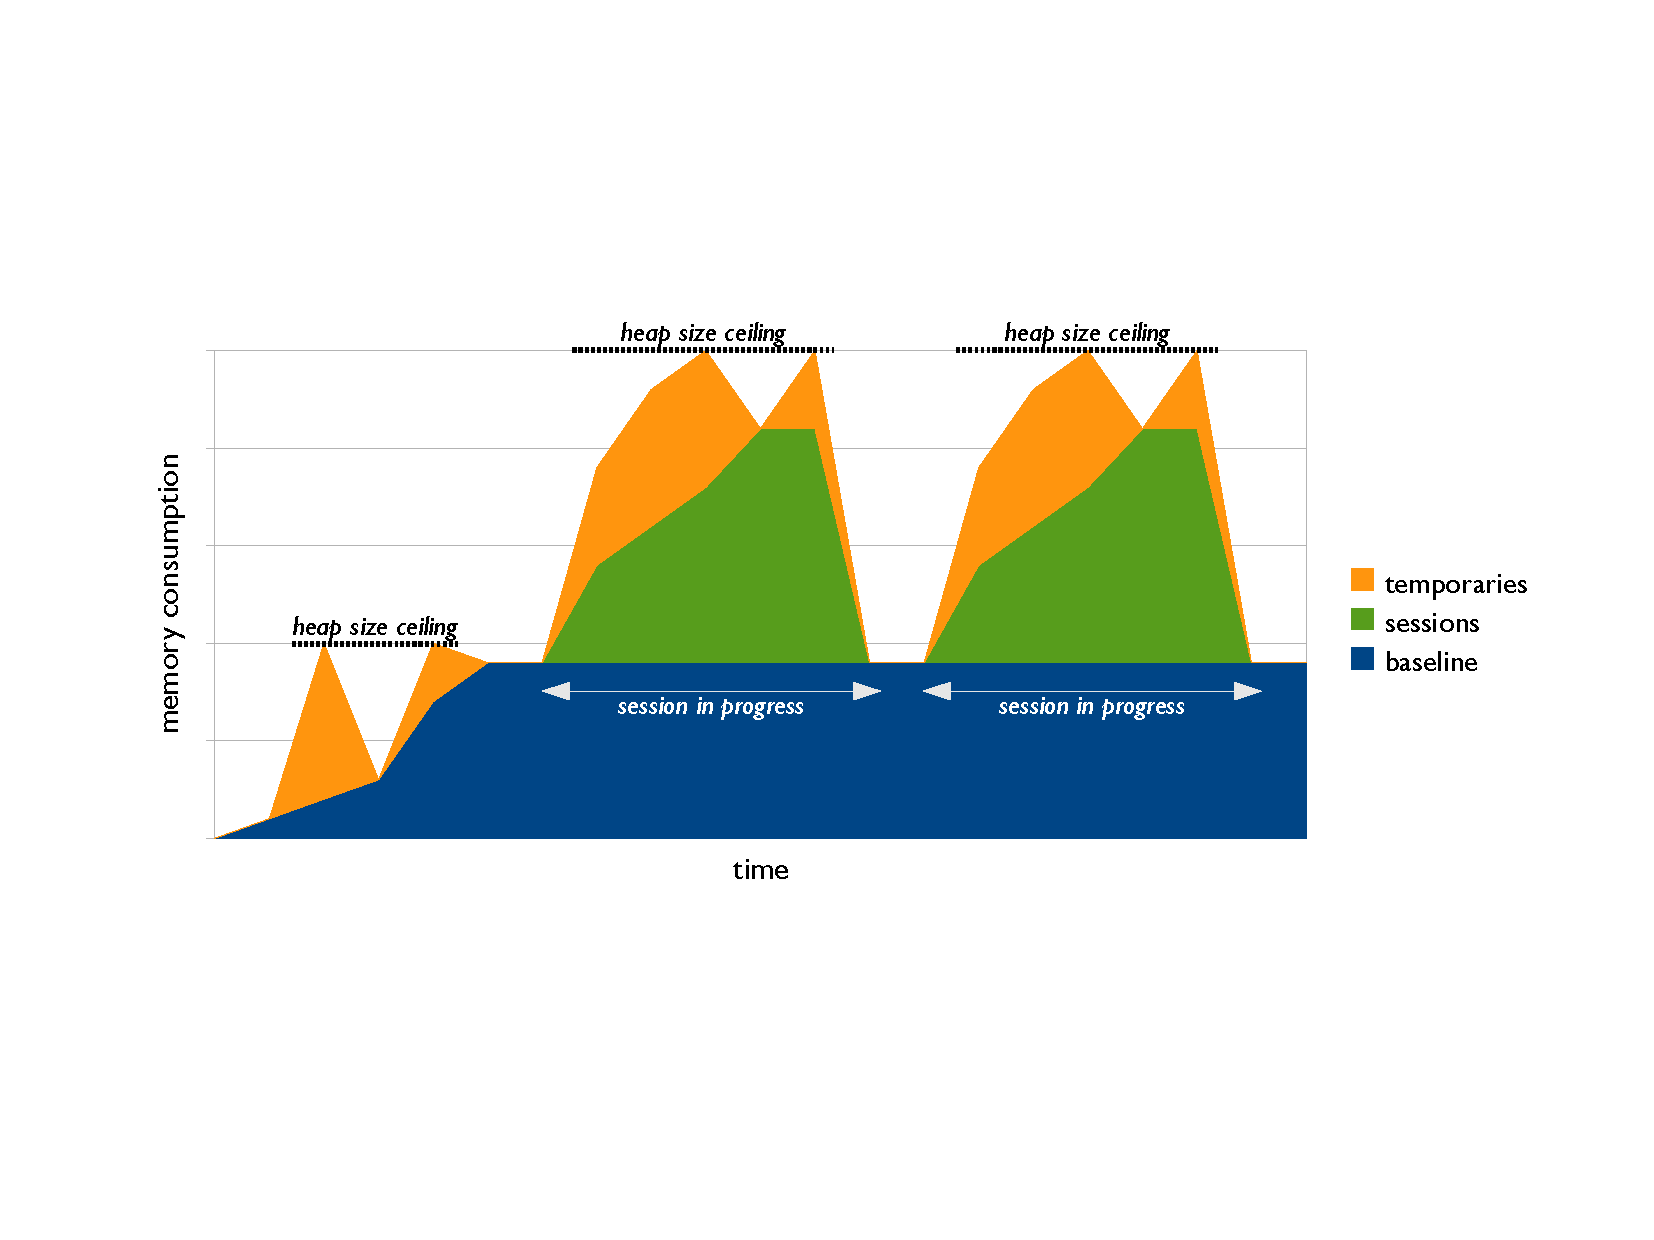
\includegraphics[width=\textwidth]{Figures/lifetime/timeline-base-session-temps}
	\caption{Memory consumption, over time, typical of a web application server.}
	\label{fig:timeline-base-session-temps}
\end{figure}

\begin{figure}
	\centering
	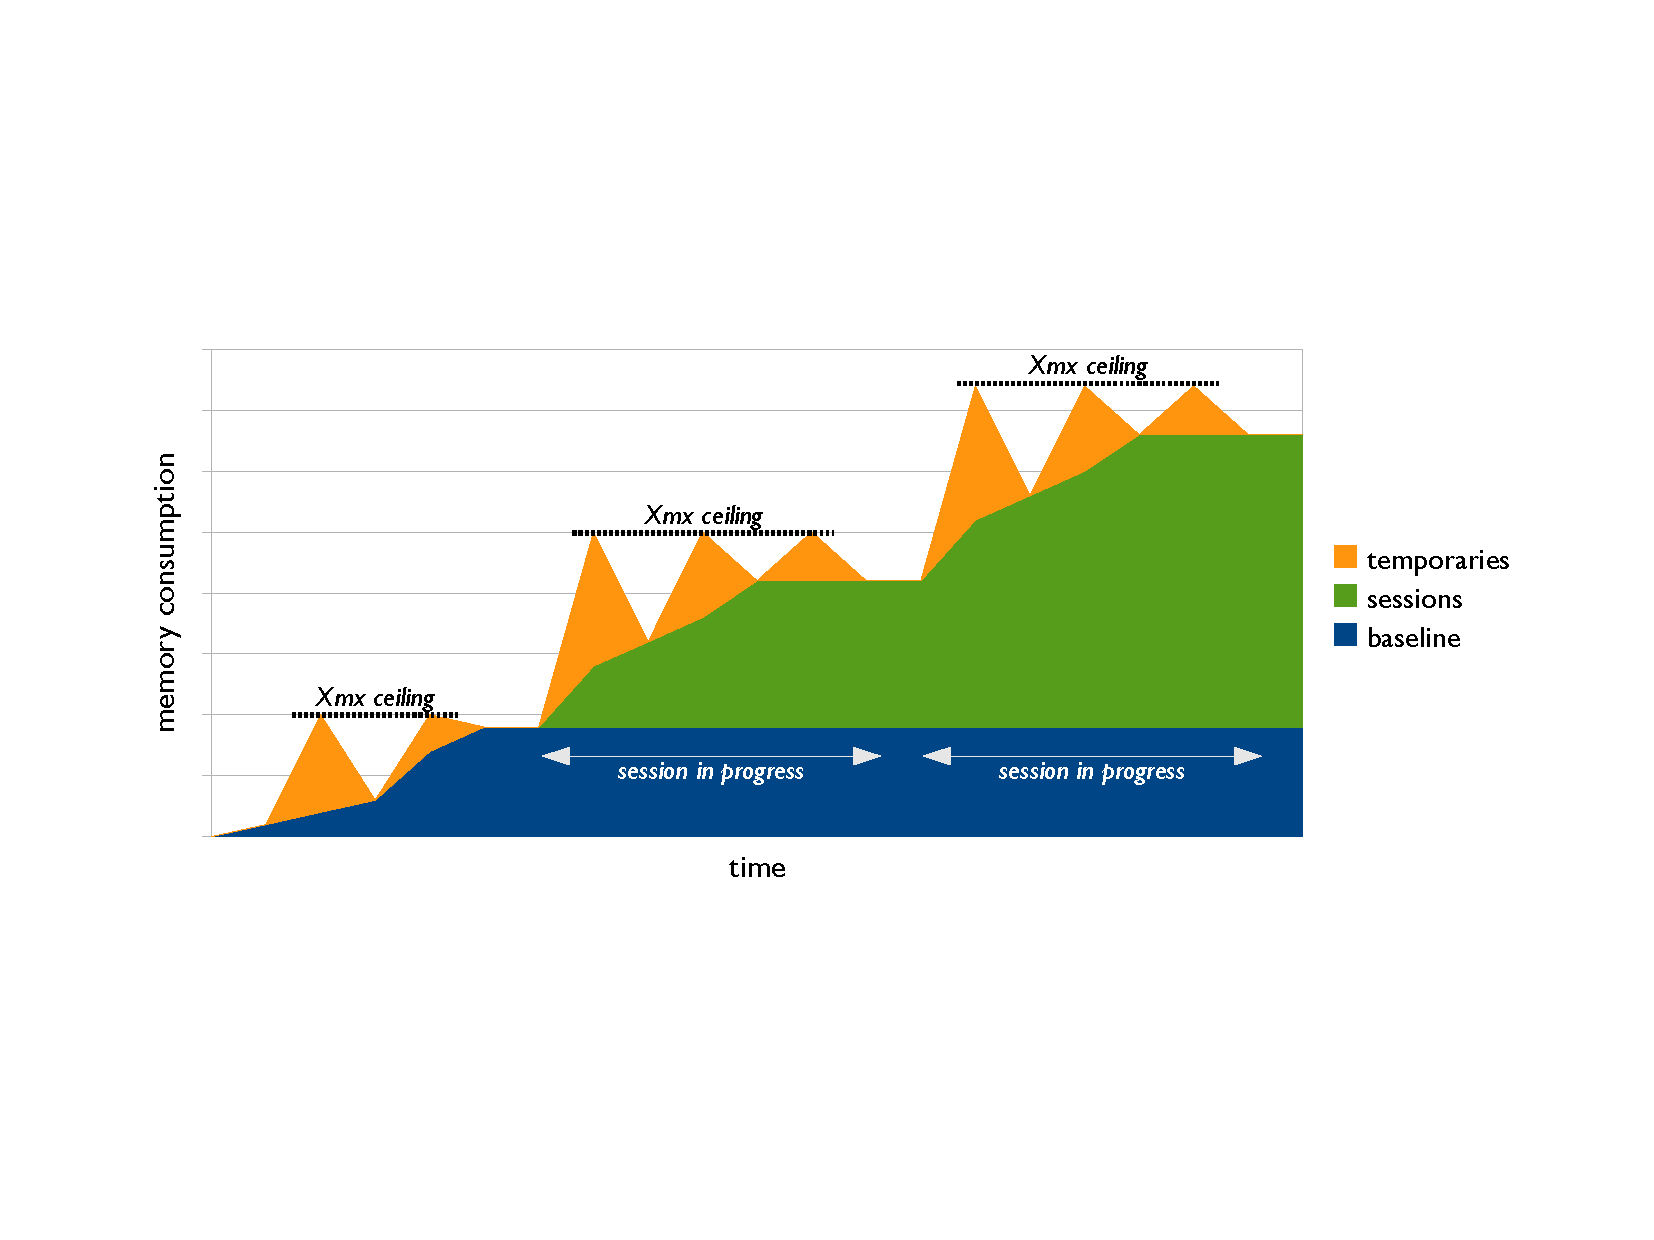
\includegraphics[width=\textwidth]{Figures/lifetime/timeline-base-session-temps-with-leak}
	\caption{If session state is not cleaned up
	properly, a memory leak is the result.}
	\label{fig:timeline-base-session-temps-with-leak}
\end{figure}

\begin{figure}
	\centering
	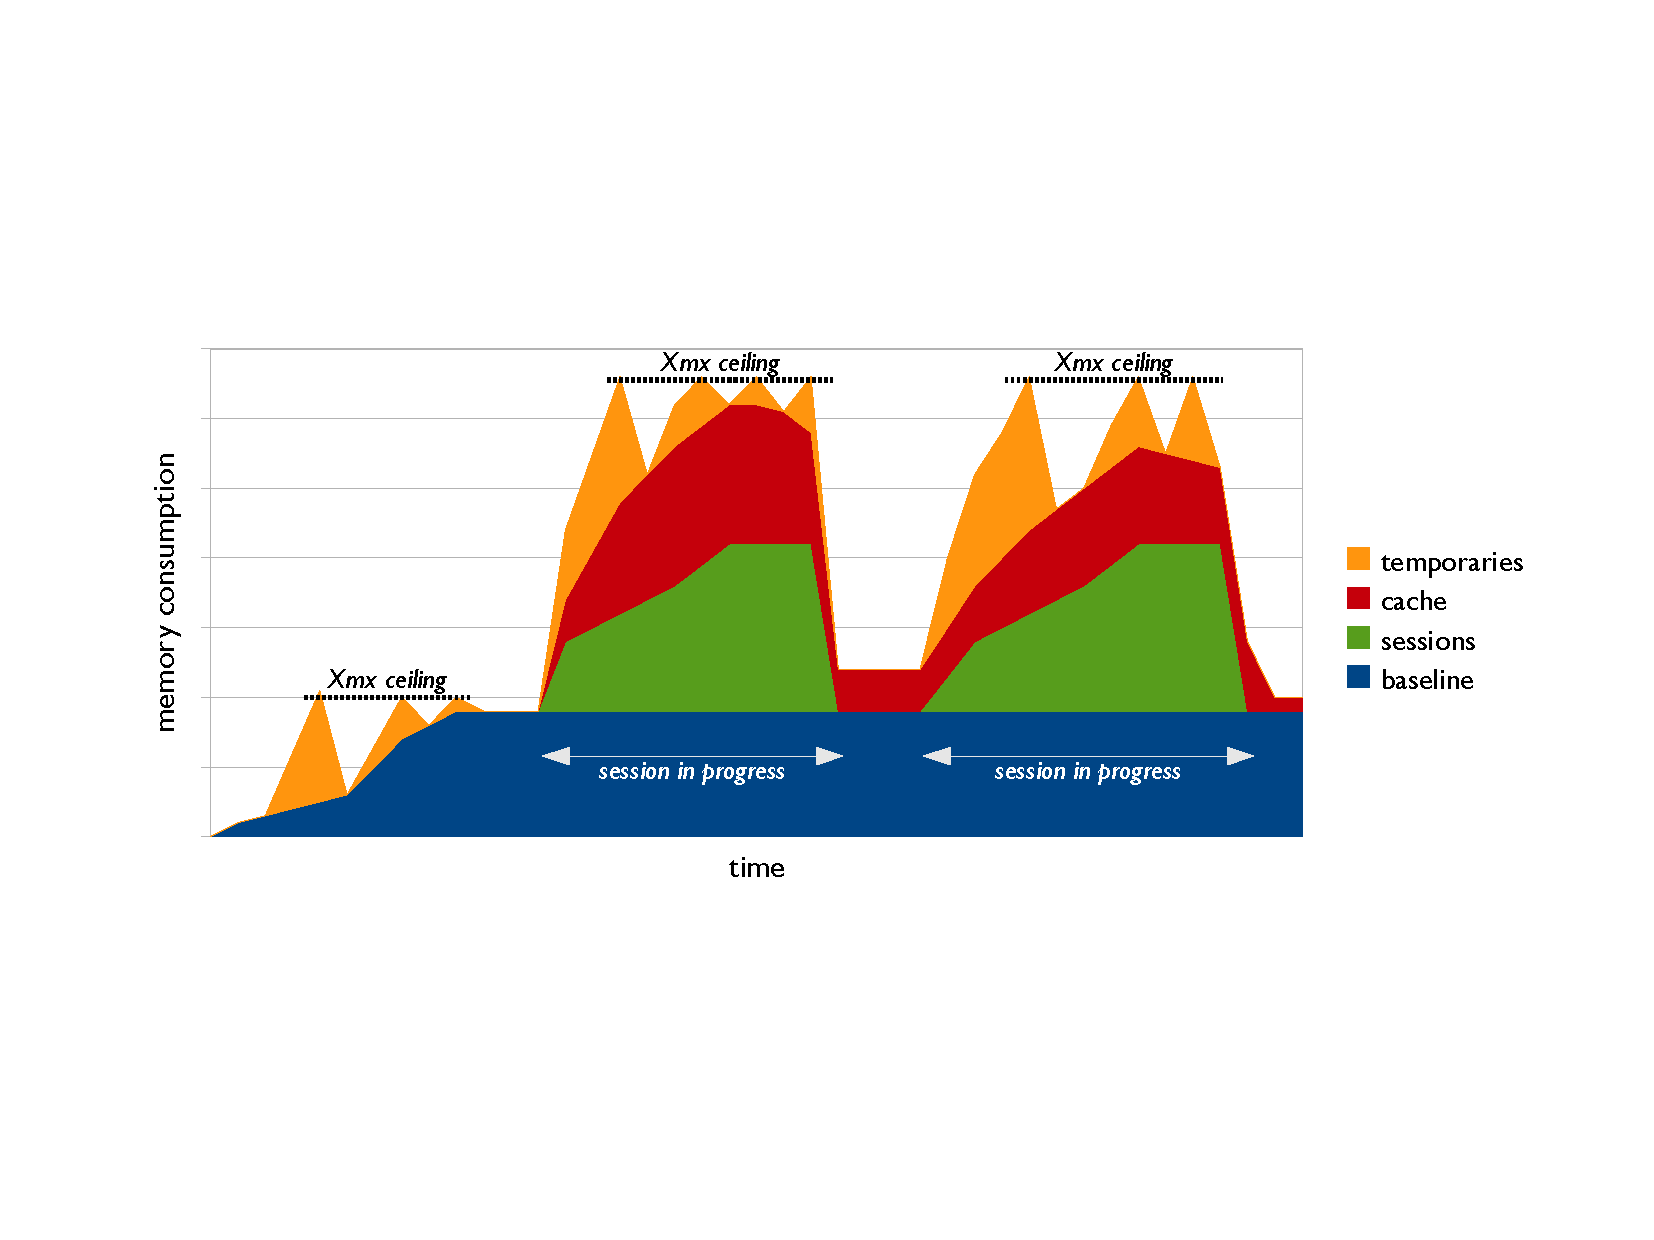
\includegraphics[width=\textwidth]{Figures/lifetime/timeline-base-session-temps-with-cache}
	\caption{When a cache is in use, this leaves less headroom for temporary
	object allocation, often resulting in more frequent garbage collections.}
	\label{fig:timeline-base-session-temps-with-cache}
\end{figure}



\begin{table}
\centering
	\begin{tabular}{lp{0.30\textwidth}p{0.35\textwidth}}
	\toprule  & Lifetime Property & Example \\ \cmidrule(r){2-2} \cmidrule(l){3-3}
	\autoref{temporary-lifetime}  & {Temporary} & new
	parser for every date
	\\
	\autoref{forever-lifetime} & {Needed Forever} & product catalog
	\\
	\autoref{correlated-lifetime-1} & {Correlated with Object}
	& object annotations
	\\
	\autoref{correlated-lifetime-2} & {Correlated with Phase} &
	DOM used only parsing
	\\
	\autoref{deferred-deletion} & {Deferred Deletion} &
	session state \\
%period\\ scoped to a phase/request\\
%correlated with an object (annotations)\\
%correlated with need}\\ \hline
%reusable & maybe i'll need it later \\ \hline
	\bottomrule
	\end{tabular}
	\caption{Five important categories of object lifetime.}
	\label{tab:five-lifetimes}
\end{table}

% introduced by example in this chapter, and
%Many objects are either temporaries or needed for
%the entire run of your application. Sometimes you create objects whose lifetime
%is correlated with other objects or that should go away when a method
%invocation completes. Sometimes you need to manage objects hanging around
%longer than their current need, to avoid future recomputations or refetching
%of data in the case when it is needed in the near future. 

\begin{table}
\centering
	\begin{tabular}{ll} \toprule
    	%& Things Java Doesn't Do Automatically \\ \cmidrule{2-2}
    	\autoref{avoiding-lifetime-bugs} & {Avoiding Memory Leaks} \\
    	\autoref{balance-time-and-space} & {Balancing Time and Space} \\
    	\autoref{outisde-java-box} & {Supporting Massive Data Sets}  	\\
        \bottomrule
    \end{tabular}
	\caption{The tricky aspects of memory management.}
	\label{tab:tricky-memory-management}
\end{table}

\section{Temporary Objects}
\label{temporary-lifetime}

If your application is like most Java applications, it creates a large number of
temporary objects. They hold data that will only be used for a very short
interval of time. For example, you populate a \class{StringBuffer}, turn it into
a \class{String}, and print the string to a log file. The point at which all of
these objects, the strings and character arrays, are no longer used is only
shortly after they are constructed. These objects serve as transient homes for
your data, as it makes its way through the frameworks and libraries you depend
on. Temporaries are often necessary to bridge separately developed code and
enable code reuse: as long as you can convert your data layout into a form that
an API requires, then you can reuse the functionality it provides.

In many cases, you need do nothing special to manage the temporary objects your
application creates. After all, generational garbage collectors these days do a
very good job digesting a large volume of temporary objects. In a generational
garbage collector, the \jre places temporary objects in a separate heap, and
thus it need only process the newly created objects during its routine scan.
Unfortunately, in Java it is pretty easy to create a high volume of temporary
objects. Say your application 
fills it the temporary heap ever second. In this case, based on the common
speeds of garbage collectors, your application could easily spend over 20\% of its time
collecting garbage.
Is it difficult to fill up the temporary heap once per second? Typical
temporary heap sizes run around 128 megabytes. Say your application is a serves
a peak of 1000 requests per second, and creates objects of around 50 bytes each.
Then it need only create around 2500 temporaries per request. 


%A great many of these
%temporary structures serve the role of a kind of lubricant, making it easy for
%you to write code that ties together the separately written parts of your code
%base and reuses standard libraries as much as possible. Often, these are
%objects that are not a fundamental necessity of what you're trying to
%accomplish. If
%you had the freedom to code highly specialized implementations of the important
%cases, from scratch, many of these temporary structures would be unnecessary.

\begin{example}{How Easy it is to Create Lots of Temporary Objects}
A common example of temporaries is parsing
and manipulating data coming from the outside world. 
% to the wire?
Consider the code in \autoref{TempExampleCode}. This code starts in
the \code{main} method by splitting the input string into two substrings. So
far, the code has created four objects (one \class{String} and one character
array per substring). 
Creating these substrings makes it easy to use the \code{doWork} method, which
takes two Strings as input. However, observe
that these four objects are not a necessary part of the computation. Indeed,
these substrings are eventually used only as input to the
\class{SimpleDateFormat} \code{parse} method, which has been nicely designed to
allow you to avoid this very problem. By passing a \class{ParsePosition}, one
can parse substrings of a string without having to create temporary strings (at
the expense of creating temporary \class{ParsePosition} objects!).
\end{example}



\begin{lstlisting}[float,caption=Code that constructs 8 temporary objects to handle two dates.,label=TempExampleCode]
void main(String xy) {
	doWork(xy.substring(0,10), xy.substring(10));
}	
void doWork(String x, String y) {
	doRemoveProcedureCall(parse(x));
	doRemoveProcedureCall(parse(y));
}
	
Date parse(String string) {
	return new SimpleDataFormat().parse(string, new ParsePosition(0));
}

void doRemoteProcedureCall(Date date) {
	long timestamp = date.getTime();
	...
}
\end{lstlisting}


% correlated with need: as soon as last user goes away, remove his stuff 
% share common expressions to save space, but using strong references -> memory
% leak; plugins in eclipse go away when all views
% sharing pool 

% weak ref keys -> annotation
% weak ref values -> sharing pool

% soft ref values -> caching

% annotation by map lookup


\section{Objects Needed Forever}
\label{forever-lifetime}

Created and used for the remaining duration of a run.


\section{Objects with Correlated Lifetimes}

Many non-temporary objects are created and then only needed for some interval of
time.

\subsection{Correlated with Another Object}
\label{correlated-lifetime-1}


For example, sometimes, you will find it necessary to associate information with
an object. You need some assurance that associated information will exit limbo
shortly after the main object does. You need their lifetimes to be {\em
correlated} with eachother. When one dies, the other should. If you can't modify
the class definition for that object, or if only a small number of objects of a
particular class need this associated information, then you'll have to store the
extra information elsewhere.

\subsection{Correlated with Invocation}
\label{correlated-lifetime-2}

Some objects should only survive as long as a phase of your program is active.
This is common, for example, if your application is an application server that
handles web requests. These server applications are often implemented as a Java
Enterprise Edition application. Let's focus on a particular example of a web
application server that handles servlet requests. In these applications, most
objects created within the scope of a servlet request will not survive the
request. Furthermore, for correctness reasons, most objects created within a
request {\em must not}, survive the request. If they unintentionally do survive,
your application has a good chance of consuming more and more memory over time.
\index{memory leak} This memory leak will eventually grind your application to a
halt, often causing it to crash. Most of these {\em request-scoped}
\index{Request-scoped Lifetime} objects are not used by the application after the
request has completed. In the absence of application or framework bugs, they will
be collected as soon as is convenient for the runtime. In this example, the
lifetime of objects during a request are {\em correlated} with a method
invocation: when the servlet \class{doGet} or \class{doPut} (etc.) invocations
return, those correlated objects had better be garbage collectible.

%\subsection{Correlated with Need} % do we need this? isn't session state a
% deferred deletion policy?
%\label{correlated-lifetime-3}

\section{Objects with Deferred-Deletion}
\label{deferred-deletion}

A cache is a performance optimization that holds on to a data structure after the
current operation is finished with it, in the hope that other operations in the
near future will reuse it. The expense of re-fetching data from external data
sources and recomputing the in-memory structure can often be amortized, at the
expense of stretching the lifetime of these data structures. By increasing the
actual lifetime on an object you will very likely increase peak memory
consumption.



%if scopes don't coincide with lifetime





%% OLD STUFF NMM 20090820
%\section{Request Scoping}
%\section{Correlated Lifetime}
%\paragraph{Weak and Soft references in Java}
%\section{Memory Leaks and Drag}
%\section{Examples}
%\subsection{Transient Near-Copies}
%\subsubsection{String Canonicalization}
%\subsection{Temporary Collections}
%\subsection{Facilitators}
